\documentclass[12pt,a4paper]{article}
\usepackage[UTF8]{ctex}
\usepackage{amsmath,amssymb}
\usepackage{xcolor}
\usepackage{hyperref}
\usepackage{geometry}
\usepackage{graphicx}
\geometry{margin=2.5cm}

\title{QAOA Maximum Independent Set / QAOA 最大独立集}
\author{QuoNic}
\date{}

\begin{document}
\maketitle

\begin{center}
\textbf{Algorithms / 算法} | 难度：高级 | 预计时间：20 分钟
\end{center}

\tableofcontents
\newpage

\section{为什么需要？}

QAOA 最大独立集是 QAOA 在图论中的经典应用。

\subsection{经典局限}
\begin{itemize}
  \item 最大独立集是 NP-hard 问题
  \item 经典算法需要指数时间
  \item 对于大规模图，经典方法效率低
\end{itemize}

\subsection{量子优势}
\begin{itemize}
  \item QAOA 可以提供比经典近似算法更好的解
  \item 对噪声有鲁棒性
  \item 理论上可以达到最优解
\end{itemize}

\subsection{实际应用}
\begin{itemize}
  \item 社交网络分析
  \item 资源分配
  \item 调度问题
\end{itemize}

\section{快速上手}

\begin{verbatim}
from quonic.algorithms import qaoa_mis

# 最大独立集
graph = [(0,1), (1,2), (2,3), (3,0)]
result = qaoa_mis(graph, p=2)
print(f'MIS size: {result.mis_size}')
print(f'MIS nodes: {result.mis_nodes}')
\end{verbatim}

\textbf{预期输出}：
\begin{verbatim}
MIS size: 2
MIS nodes: [0, 2]
\end{verbatim}

\section{原理详解}

\subsection{电路图}

\begin{center}
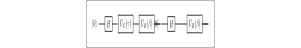
\includegraphics[width=0.6\textwidth]{../../images/qaoa_mis_circuit.svg}
\end{center}

\subsection{数学推导}

最大独立集问题：
\begin{equation}
\max \sum_i x_i \quad \text{s.t.} \quad x_i + x_j \leq 1, \forall (i,j) \in E
\end{equation}

QAOA 编码：
\begin{equation}
C(x) = \sum_i x_i - \lambda \sum_{(i,j) \in E} x_i x_j
\end{equation}

其中 $\lambda$ 是惩罚系数。

\subsection{几何解释}

QAOA 最大独立集在参数空间中寻找最大独立集。量子计算机负责制备态和测量，经典优化器负责更新参数。

\section{代码详解}

\begin{verbatim}
from quonic.algorithms import qaoa_mis

# qaoa_mis(graph, p, optimizer)
# graph: 图的边列表
# p: QAOA 层数
# optimizer: 优化器

result = qaoa_mis(
    graph=[(0,1), (1,2), (2,3), (3,0)],
    p=2,
    optimizer='cobyla'
)

# result.mis_size: 最大独立集大小
# result.mis_nodes: 最大独立集节点
# result.params: 优化后的参数
print(f'MIS size: {result.mis_size}')
print(f'MIS nodes: {result.mis_nodes}')
\end{verbatim}

\section{进阶用法}

\subsection{场景 1：不同层数}

\begin{verbatim}
from quonic.algorithms import qaoa_mis

graph = [(0,1), (1,2), (2,3), (3,0)]

for p in [1, 2, 4]:
    result = qaoa_mis(graph, p=p)
    print(f'p={p}: MIS size={result.mis_size}')
\end{verbatim}

\subsection{场景 2：不同图}

\begin{verbatim}
from quonic.algorithms import qaoa_mis

# 不同图
graph1 = [(0,1), (1,2), (2,0)]  # 三角形
graph2 = [(0,1), (1,2), (2,3), (3,0)]  # 正方形
graph3 = [(0,1), (0,2), (0,3), (1,2), (1,3), (2,3)]  # 完全图

for graph in [graph1, graph2, graph3]:
    result = qaoa_mis(graph, p=2)
    print(f'MIS size: {result.mis_size}')
\end{verbatim}

\subsection{场景 3：大规模图}

\begin{verbatim}
from quonic.algorithms import qaoa_mis
import networkx as nx

# 大规模图
G = nx.erdos_renyi_graph(20, 0.3)
graph = list(G.edges())

result = qaoa_mis(graph, p=3)
print(f'MIS size: {result.mis_size}')
\end{verbatim}

\section{适用场景}

\subsection{社交网络分析}

QAOA 最大独立集可以用于社交网络中的社区检测。最大独立集对应社交网络中互不相识的用户群。

\subsection{资源分配}

QAOA 最大独立集可以用于资源分配。例如，在有限资源下选择互不冲突的任务。

\section{常见问题}

\subsection{QAOA 最大独立集和经典最大独立集有什么区别？}

QAOA 最大独立集使用量子策略，可以利用量子叠加探索更大的解空间。

\subsection{QAOA 最大独立集的精度如何？}

精度取决于层数和参数优化策略。

\section{学习路径}

\subsection{前置知识}
\begin{itemize}
  \item QAOA
  \item 图论
  \item 独立集
\end{itemize}

\subsection{继续学习}
\begin{itemize}
  \item QAOA MaxCut
  \item QAOA 背包问题
  \item 量子优化
\end{itemize}

\section{完整示例代码}

\subsection{示例 1：基本 QAOA 最大独立集}

\begin{verbatim}
from quonic.algorithms import qaoa_mis

graph = [(0,1), (1,2), (2,3), (3,0)]
result = qaoa_mis(graph, p=2)
print(f'MIS size: {result.mis_size}')
\end{verbatim}

\section{下载}

\begin{itemize}
  \item [qaoa\_mis.py](https://github.com/ChrisLee0721/QuoNic/blob/main/examples/qaoa_mis/qaoa_mis.py)
\end{itemize}

\end{document}
